\section{Experiments}
\label{sec:experiments}

\subsection{Datasets and Experimental Settings}
\label{sec:experimental_settings}

% 按作者提供的原文录入，仅转换为共享中英文稿所需的 LaTeX 格式。
\paragraph{Datasets.}
We evaluate ALM-MIL on four real-world clinical cohorts and four public medical imaging benchmarks. The clinical cohorts comprise white-light endoscopy (WLE; 977 examinations, 79,508 images), chromoendoscopy (340 examinations, 29,439 images), surgical gastroscopy (965 examinations, 43,706 images), and endoscopic ultrasonography (EUS; 579 examinations, 18,938 images), all using a three-label setting. The public benchmarks cover different examination types: the chest CT--radiology-report benchmark (CT-RATE) includes 680 examinations, 157,702 slices, and 3 target labels; the brain-and-spine MRI benchmark (MR-RATE-1K) includes 1,000 examinations, 832,672 slices, and 4 target labels; the Abdominal Multimodal Analysis Challenge dataset (AMOS-MM) includes CT examinations spanning the chest, abdomen, and pelvis, with 1,686 examinations, 268,024 slices, and 7 target labels; and the AbdomenAtlas 3.0 Mini abdominal CT dataset (AA-Mini) includes 9,261 examinations and 3 target labels. Each examination consists of an ordered image sequence, a paired findings report with target-label information masked, and examination-level multi-label annotations.

\cntranslation{%
\textbf{数据集。} 我们在四个真实临床队列和四个公开医学影像基准上评估 ALM-MIL。四个真实临床队列包括白光胃镜（WLE；977 次检查，79,508 张图像）、染色胃镜（340 次检查，29,439 张图像）、手术胃镜（965 次检查，43,706 张图像）以及超声胃镜（EUS；579 次检查，18,938 张图像），四个队列均采用三标签设置。四个公开基准覆盖不同的检查类型：胸部 CT 放射学报告基准（CT-RATE）包含 680 次检查、157,702 张切片和 3 个目标标签；脑部与脊柱 MRI 基准（MR-RATE-1K）包含 1,000 次检查、832,672 张切片和 4 个目标标签；腹部多模态分析挑战赛数据集（AMOS-MM）包含覆盖胸部、腹部和盆腔的 CT 检查，共 1,686 次检查、268,024 张切片和 7 个目标标签；AbdomenAtlas 3.0 Mini 腹部 CT 数据集（AA-Mini）包含 9,261 次检查和 3 个目标标签。每次检查由一组有序图像、一份遮蔽目标标签信息的配对所见报告以及检查级多标签标注组成。
}

\paragraph{Experimental Settings.}
All experiments follow a five-fold evaluation protocol. For all datasets, data are split at the patient level, with three folds used for training, one for validation, and one for testing in each run. We uniformly sample up to 64 images from each examination while preserving the original acquisition order and resize them to \(224\times224\). A pretrained ConvNeXt-Tiny serves as the visual encoder, while the masked findings report is encoded by a multi-scale TextCNN. Models are optimized with AdamW for up to 30 epochs, using an initial learning rate of \(2\times10^{-5}\) and a weight decay of 0.02. Macro-F1 is used as the primary evaluation metric, hereafter denoted as F1. For each fold, we select the model with the highest validation F1 and evaluate it on the corresponding test fold. Final results are reported as the mean and standard deviation over five folds. Additional implementation details are provided in the Appendix.

\cntranslation{%
\textbf{实验设置。} 所有实验均采用五折评估协议。对于所有数据集，我们均按照患者进行分组划分，每轮使用三折训练、一折验证和一折测试。每次检查按照原始采集顺序最多均匀采样 64 张图像，并统一缩放至 \(224\times224\)。视觉端采用预训练的 ConvNeXt-Tiny 作为编码器，遮蔽目标标签信息后的所见报告采用多尺度 TextCNN 编码。模型使用 AdamW 优化，最多训练 30 个 epoch，初始学习率设为 \(2\times10^{-5}\)，weight decay 为 0.02。我们采用 Macro-F1 作为主要评价指标，后文简称为 F1。每折选取验证集 F1 最高的模型，并在对应测试折上进行评估，最终报告五折结果的均值和标准差。其余实现细节见附录。
}

\subsection{Overall Performance Comparison}
\label{sec:overall_comparison}

% 作者指定的待确认草稿：暂按 ALM-MIL 在七个数据集上均取得最优 F1 的假设行文。
% 表格中的全部结果仍为占位符；该假设须在最终实验结果确定后核对。
\begin{table*}[t]
\centering
\caption{Overall comparison on four clinical cohorts and four public datasets (F1, \%).
Img. and Txt. indicate image and report inputs, respectively. WLE, Chromo.,
Surg., and EUS denote white-light endoscopy, chromoendoscopy, surgical
gastroscopy, and endoscopic ultrasonography, respectively.}
\label{tab:overall_comparison}
\cntranslation{%
四个临床队列和四个公开数据集上的总体比较（F1，\%）。Img. 和 Txt. 分别表示图像与报告输入；WLE、Chromo.、Surg. 和 EUS 分别表示白光胃镜、染色胃镜、手术胃镜和超声胃镜。
}
\setlength{\tabcolsep}{1.8pt}
\renewcommand{\arraystretch}{1.08}
\fontsize{8.2}{9.3}\selectfont
\begin{tabular*}{\textwidth}{@{\extracolsep{\fill}}l|cc|cccc|cccc@{}}
\toprule
Model & Img. & Txt. & WLE & Chromo. & Surg. & EUS & CT-RATE & MR-RATE-1K & AMOS-MM & AA-Mini \\
\midrule
Attention MIL & $\checkmark$ & $\times$ & 79.19\scalebox{0.6667}{$\pm$1.19} & 73.91\scalebox{0.6667}{$\pm$4.48} & 70.18\scalebox{0.6667}{$\pm$12.35} & 62.68\scalebox{0.6667}{$\pm$3.42} & 43.38\scalebox{0.6667}{$\pm$2.32} & 61.78\scalebox{0.6667}{$\pm$2.25} & 41.07\scalebox{0.6667}{$\pm$0.00} & 49.43\scalebox{0.6667}{$\pm$0.84} \\
TransMIL & $\checkmark$ & $\times$ & 80.21\scalebox{0.6667}{$\pm$1.46} & 72.17\scalebox{0.6667}{$\pm$3.68} & 75.16\scalebox{0.6667}{$\pm$9.38} & 60.45\scalebox{0.6667}{$\pm$5.39} & 43.58\scalebox{0.6667}{$\pm$1.90} & 60.15\scalebox{0.6667}{$\pm$0.75} & 40.27\scalebox{0.6667}{$\pm$1.04} & 49.47\scalebox{0.6667}{$\pm$1.18} \\
DSMIL & $\checkmark$ & $\times$ & 79.56\scalebox{0.6667}{$\pm$1.59} & 74.68\scalebox{0.6667}{$\pm$4.48} & 68.73\scalebox{0.6667}{$\pm$8.52} & 57.65\scalebox{0.6667}{$\pm$7.65} & 43.79\scalebox{0.6667}{$\pm$2.18} & 60.86\scalebox{0.6667}{$\pm$2.09} & 40.17\scalebox{0.6667}{$\pm$1.38} & 48.69\scalebox{0.6667}{$\pm$1.45} \\
DTFD-MIL & $\checkmark$ & $\times$ & 77.14\scalebox{0.6667}{$\pm$1.41} & 70.91\scalebox{0.6667}{$\pm$3.06} & 71.34\scalebox{0.6667}{$\pm$8.53} & 58.96\scalebox{0.6667}{$\pm$4.19} & 43.94\scalebox{0.6667}{$\pm$1.67} & 62.18\scalebox{0.6667}{$\pm$1.82} & 40.79\scalebox{0.6667}{$\pm$0.78} & 49.25\scalebox{0.6667}{$\pm$1.28} \\
CLAM-MB & $\checkmark$ & $\times$ & 77.41\scalebox{0.6667}{$\pm$0.90} & 71.37\scalebox{0.6667}{$\pm$2.69} & 70.94\scalebox{0.6667}{$\pm$8.65} & 58.83\scalebox{0.6667}{$\pm$4.01} & 44.24\scalebox{0.6667}{$\pm$1.36} & 50.84\scalebox{0.6667}{$\pm$1.40} & 39.14\scalebox{0.6667}{$\pm$0.03} & 47.35\scalebox{0.6667}{$\pm$0.78} \\
CLAM-SB & $\checkmark$ & $\times$ & 76.42\scalebox{0.6667}{$\pm$0.40} & 69.97\scalebox{0.6667}{$\pm$2.34} & 67.85\scalebox{0.6667}{$\pm$4.79} & 56.95\scalebox{0.6667}{$\pm$3.79} & 43.98\scalebox{0.6667}{$\pm$1.10} & 53.54\scalebox{0.6667}{$\pm$4.47} & 39.62\scalebox{0.6667}{$\pm$0.50} & 43.95\scalebox{0.6667}{$\pm$1.95} \\
GCF-Net$^{\dagger}$ & $\checkmark$ & $\times$ & 83.40\scalebox{0.6667}{$\pm$1.09} & 72.60\scalebox{0.6667}{$\pm$6.35} & 70.84\scalebox{0.6667}{$\pm$9.75} & 61.10\scalebox{0.6667}{$\pm$3.42} & 44.74\scalebox{0.6667}{$\pm$3.01} & 59.98\scalebox{0.6667}{$\pm$1.36} & 40.59\scalebox{0.6667}{$\pm$0.80} & 49.99\scalebox{0.6667}{$\pm$1.05} \\
\midrule
Hashed mean & $\times$ & $\checkmark$ & 88.01\scalebox{0.6667}{$\pm$1.84} & 79.37\scalebox{0.6667}{$\pm$6.89} & 82.49\scalebox{0.6667}{$\pm$1.87} & 87.36\scalebox{0.6667}{$\pm$6.88} & 60.91\scalebox{0.6667}{$\pm$2.93} & 67.92\scalebox{0.6667}{$\pm$2.29} & 45.62\scalebox{0.6667}{$\pm$2.08} & 64.41\scalebox{0.6667}{$\pm$0.91} \\
Vocabulary attention & $\times$ & $\checkmark$ & 88.06\scalebox{0.6667}{$\pm$1.24} & 79.45\scalebox{0.6667}{$\pm$7.08} & 80.47\scalebox{0.6667}{$\pm$4.87} & 88.57\scalebox{0.6667}{$\pm$5.42} & 72.34\scalebox{0.6667}{$\pm$3.15} & 70.54\scalebox{0.6667}{$\pm$2.55} & 49.13\scalebox{0.6667}{$\pm$2.37} & 65.53\scalebox{0.6667}{$\pm$0.81} \\
TextCNN & $\times$ & $\checkmark$ & 89.04\scalebox{0.6667}{$\pm$1.23} & 85.52\scalebox{0.6667}{$\pm$3.32} & 82.56\scalebox{0.6667}{$\pm$8.07} & 88.82\scalebox{0.6667}{$\pm$5.15} & 67.88\scalebox{0.6667}{$\pm$6.15} & 69.45\scalebox{0.6667}{$\pm$0.76} & 49.66\scalebox{0.6667}{$\pm$0.83} & 67.16\scalebox{0.6667}{$\pm$1.06} \\
BiGRU & $\times$ & $\checkmark$ & 88.28\scalebox{0.6667}{$\pm$1.91} & 79.85\scalebox{0.6667}{$\pm$8.18} & 79.75\scalebox{0.6667}{$\pm$3.42} & 89.19\scalebox{0.6667}{$\pm$5.31} & 62.69\scalebox{0.6667}{$\pm$1.86} & 68.31\scalebox{0.6667}{$\pm$1.61} & 46.30\scalebox{0.6667}{$\pm$0.72} & 66.04\scalebox{0.6667}{$\pm$0.94} \\
Transformer & $\times$ & $\checkmark$ & 88.15\scalebox{0.6667}{$\pm$1.63} & 80.50\scalebox{0.6667}{$\pm$2.81} & 81.85\scalebox{0.6667}{$\pm$1.74} & 87.30\scalebox{0.6667}{$\pm$6.04} & 76.50\scalebox{0.6667}{$\pm$2.59} & 69.56\scalebox{0.6667}{$\pm$0.02} & 48.45\scalebox{0.6667}{$\pm$1.59} & 64.96\scalebox{0.6667}{$\pm$1.66} \\
\midrule
MMFNet$^{\dagger}$ & $\checkmark$ & $\checkmark$ & 91.32\scalebox{0.6667}{$\pm$0.99} & 83.71\scalebox{0.6667}{$\pm$6.47} & 83.45\scalebox{0.6667}{$\pm$8.44} & 89.99\scalebox{0.6667}{$\pm$7.31} & 57.34\scalebox{0.6667}{$\pm$2.37} & 70.17\scalebox{0.6667}{$\pm$2.26} & 45.76\scalebox{0.6667}{$\pm$3.01} & 72.33\scalebox{0.6667}{$\pm$1.37} \\
RadFuse$^{\dagger}$ & $\checkmark$ & $\checkmark$ & 91.35\scalebox{0.6667}{$\pm$0.83} & 79.90\scalebox{0.6667}{$\pm$10.13} & 82.21\scalebox{0.6667}{$\pm$6.71} & 85.17\scalebox{0.6667}{$\pm$7.12} & 67.88\scalebox{0.6667}{$\pm$4.39} & 66.58\scalebox{0.6667}{$\pm$2.08} & 41.73\scalebox{0.6667}{$\pm$0.93} & 62.00\scalebox{0.6667}{$\pm$2.17} \\
SAIF$^{\dagger}$ & $\checkmark$ & $\checkmark$ & 84.13\scalebox{0.6667}{$\pm$1.66} & 72.01\scalebox{0.6667}{$\pm$5.44} & 74.82\scalebox{0.6667}{$\pm$8.21} & 62.66\scalebox{0.6667}{$\pm$9.86} & 44.81\scalebox{0.6667}{$\pm$2.00} & 60.86\scalebox{0.6667}{$\pm$1.55} & 40.84\scalebox{0.6667}{$\pm$0.53} & 67.47\scalebox{0.6667}{$\pm$3.14} \\
MMTF$^{\dagger}$ & $\checkmark$ & $\checkmark$ & 91.21\scalebox{0.6667}{$\pm$1.18} & 73.20\scalebox{0.6667}{$\pm$4.15} & 75.95\scalebox{0.6667}{$\pm$13.71} & 78.46\scalebox{0.6667}{$\pm$9.74} & 77.79\scalebox{0.6667}{$\pm$4.02} & 73.88\scalebox{0.6667}{$\pm$0.23} & 49.20\scalebox{0.6667}{$\pm$1.75} & 74.42\scalebox{0.6667}{$\pm$1.57} \\
CaMCheX$^{\dagger}$ & $\checkmark$ & $\checkmark$ & 90.87\scalebox{0.6667}{$\pm$3.41} & 83.16\scalebox{0.6667}{$\pm$5.28} & 83.39\scalebox{0.6667}{$\pm$6.17} & 89.12\scalebox{0.6667}{$\pm$4.96} & 78.83\scalebox{0.6667}{$\pm$5.67} & 69.20\scalebox{0.6667}{$\pm$1.69} & 52.94\scalebox{0.6667}{$\pm$2.00} & 73.95\scalebox{0.6667}{$\pm$1.50} \\
Med3DVLM$^{\dagger}$ & $\checkmark$ & $\checkmark$ & 88.43\scalebox{0.6667}{$\pm$2.76} & 79.24\scalebox{0.6667}{$\pm$6.13} & 80.15\scalebox{0.6667}{$\pm$7.32} & 88.68\scalebox{0.6667}{$\pm$5.87} & 72.85\scalebox{0.6667}{$\pm$3.41} & 71.98\scalebox{0.6667}{$\pm$0.36} & 51.65\scalebox{0.6667}{$\pm$5.37} & \textbf{74.43\scalebox{0.6667}{$\pm$0.73}} \\
M3FM$^{\dagger}$ & $\checkmark$ & $\checkmark$ & 87.61\scalebox{0.6667}{$\pm$3.18} & 80.89\scalebox{0.6667}{$\pm$4.75} & 79.46\scalebox{0.6667}{$\pm$6.84} & 86.17\scalebox{0.6667}{$\pm$5.41} & 72.48\scalebox{0.6667}{$\pm$4.43} & 68.58\scalebox{0.6667}{$\pm$1.06} & 48.39\scalebox{0.6667}{$\pm$1.25} & 72.85\scalebox{0.6667}{$\pm$1.01} \\
Unified MM$^{\dagger}$ & $\checkmark$ & $\checkmark$ & 90.98\scalebox{0.6667}{$\pm$0.65} & 85.01\scalebox{0.6667}{$\pm$5.00} & 84.44\scalebox{0.6667}{$\pm$8.82} & 90.12\scalebox{0.6667}{$\pm$5.36} & 69.00\scalebox{0.6667}{$\pm$7.85} & 69.74\scalebox{0.6667}{$\pm$3.58} & 47.89\scalebox{0.6667}{$\pm$2.50} & 74.10\scalebox{0.6667}{$\pm$1.39} \\
Adaptive Fusion$^{\dagger\ddagger}$ & $\checkmark$ & $\checkmark$ & 89.72\scalebox{0.6667}{$\pm$0.73} & 84.90\scalebox{0.6667}{$\pm$4.79} & 81.43\scalebox{0.6667}{$\pm$5.69} & 89.16\scalebox{0.6667}{$\pm$7.45} & 71.03\scalebox{0.6667}{$\pm$5.74} & 72.35\scalebox{0.6667}{$\pm$1.45} & 50.24\scalebox{0.6667}{$\pm$2.67} & 73.26\scalebox{0.6667}{$\pm$0.73} \\
\midrule
\textbf{ALM-MIL (Ours)} & $\checkmark$ & $\checkmark$ & \textbf{91.49\scalebox{0.6667}{$\pm$1.14}} & \textbf{88.77\scalebox{0.6667}{$\pm$1.68}} & \textbf{84.56\scalebox{0.6667}{$\pm$2.24}} & \textbf{90.64\scalebox{0.6667}{$\pm$4.74}} & \textbf{81.34\scalebox{0.6667}{$\pm$1.86}} & \textbf{74.45\scalebox{0.6667}{$\pm$1.93}} & \textbf{54.12\scalebox{0.6667}{$\pm$3.12}} & 73.85\scalebox{0.6667}{$\pm$1.79} \\
\bottomrule
\end{tabular*}

\vspace{2pt}
\begin{minipage}{\textwidth}
\footnotesize
$^{\dagger}$ denotes methods adapted or reimplemented for the present task;
$^{\ddagger}$ denotes a preprint. Unified MM and Adaptive Fusion abbreviate
Unified Multimodal Framework and Adaptive Multimodal Fusion, respectively.
\cntranslation{%
$^{\dagger}$ 表示针对当前任务适配或重新实现的方法；$^{\ddagger}$ 表示预印本。Unified MM 和 Adaptive Fusion 分别简称 Unified Multimodal Framework 和 Adaptive Multimodal Fusion。
}
\end{minipage}
\end{table*}

We compare ALM-MIL with image-only, text-only, and multimodal baselines on all eight datasets, as summarized in Table~\ref{tab:overall_comparison}. Across the four clinical cohorts and three of the four public datasets, ALM-MIL achieves the highest mean F1, outperforming both unimodal and multimodal baselines. On AA-Mini, its performance is lower than Med3DVLM and other multimodal baselines. This may be related to the weak co-occurrence correlations among AA-Mini's target labels, which provide limited relational information for LCCF to exploit and thus leave less room for further classification gains. Overall, the leading results achieved by our model on these endoscopic, CT, and MRI examinations support the applicability of the framework across imaging modalities and target-label configurations. The following sections examine the contributions of ACPE and LCCF through targeted analyses.

\cntranslation{%
我们在全部八个数据集上，将 ALM-MIL 与纯图像、纯文本及多模态基线进行比较，结果汇总于表~\ref{tab:overall_comparison}。ALM-MIL 在四个临床队列和四个公开数据集中的三个数据集上取得最高的平均 F1，优于纯图像、纯文本及多模态基线。在 AA-Mini 上，其性能低于 Med3DVLM 等多模态基线。这可能与 AA-Mini 各目标标签之间较弱的共现相关性有关：标签关系能够提供的互补信息有限，因此 LCCF 可利用的关系信息较少，难以进一步提升分类性能。总体而言，我们的模型在这些内镜、CT 和 MRI 检查中取得的领先结果支持了该框架在不同成像模态与目标标签设置下的适用性。后续章节将通过针对性分析，进一步考察 ACPE 和 LCCF 的贡献。
}

\subsection{Robustness under Structured Image Missingness}
\label{sec:structured_missingness}

% 当前图件：fig/fig3.pdf。
% 数据依据作者指定的 r051_3d_figure_data.csv；保留原脚本样式。
% 第八种条件按作者指定标注为 Rand.；图件后续仍可替换。
\begin{figure}[t]
    \centering
    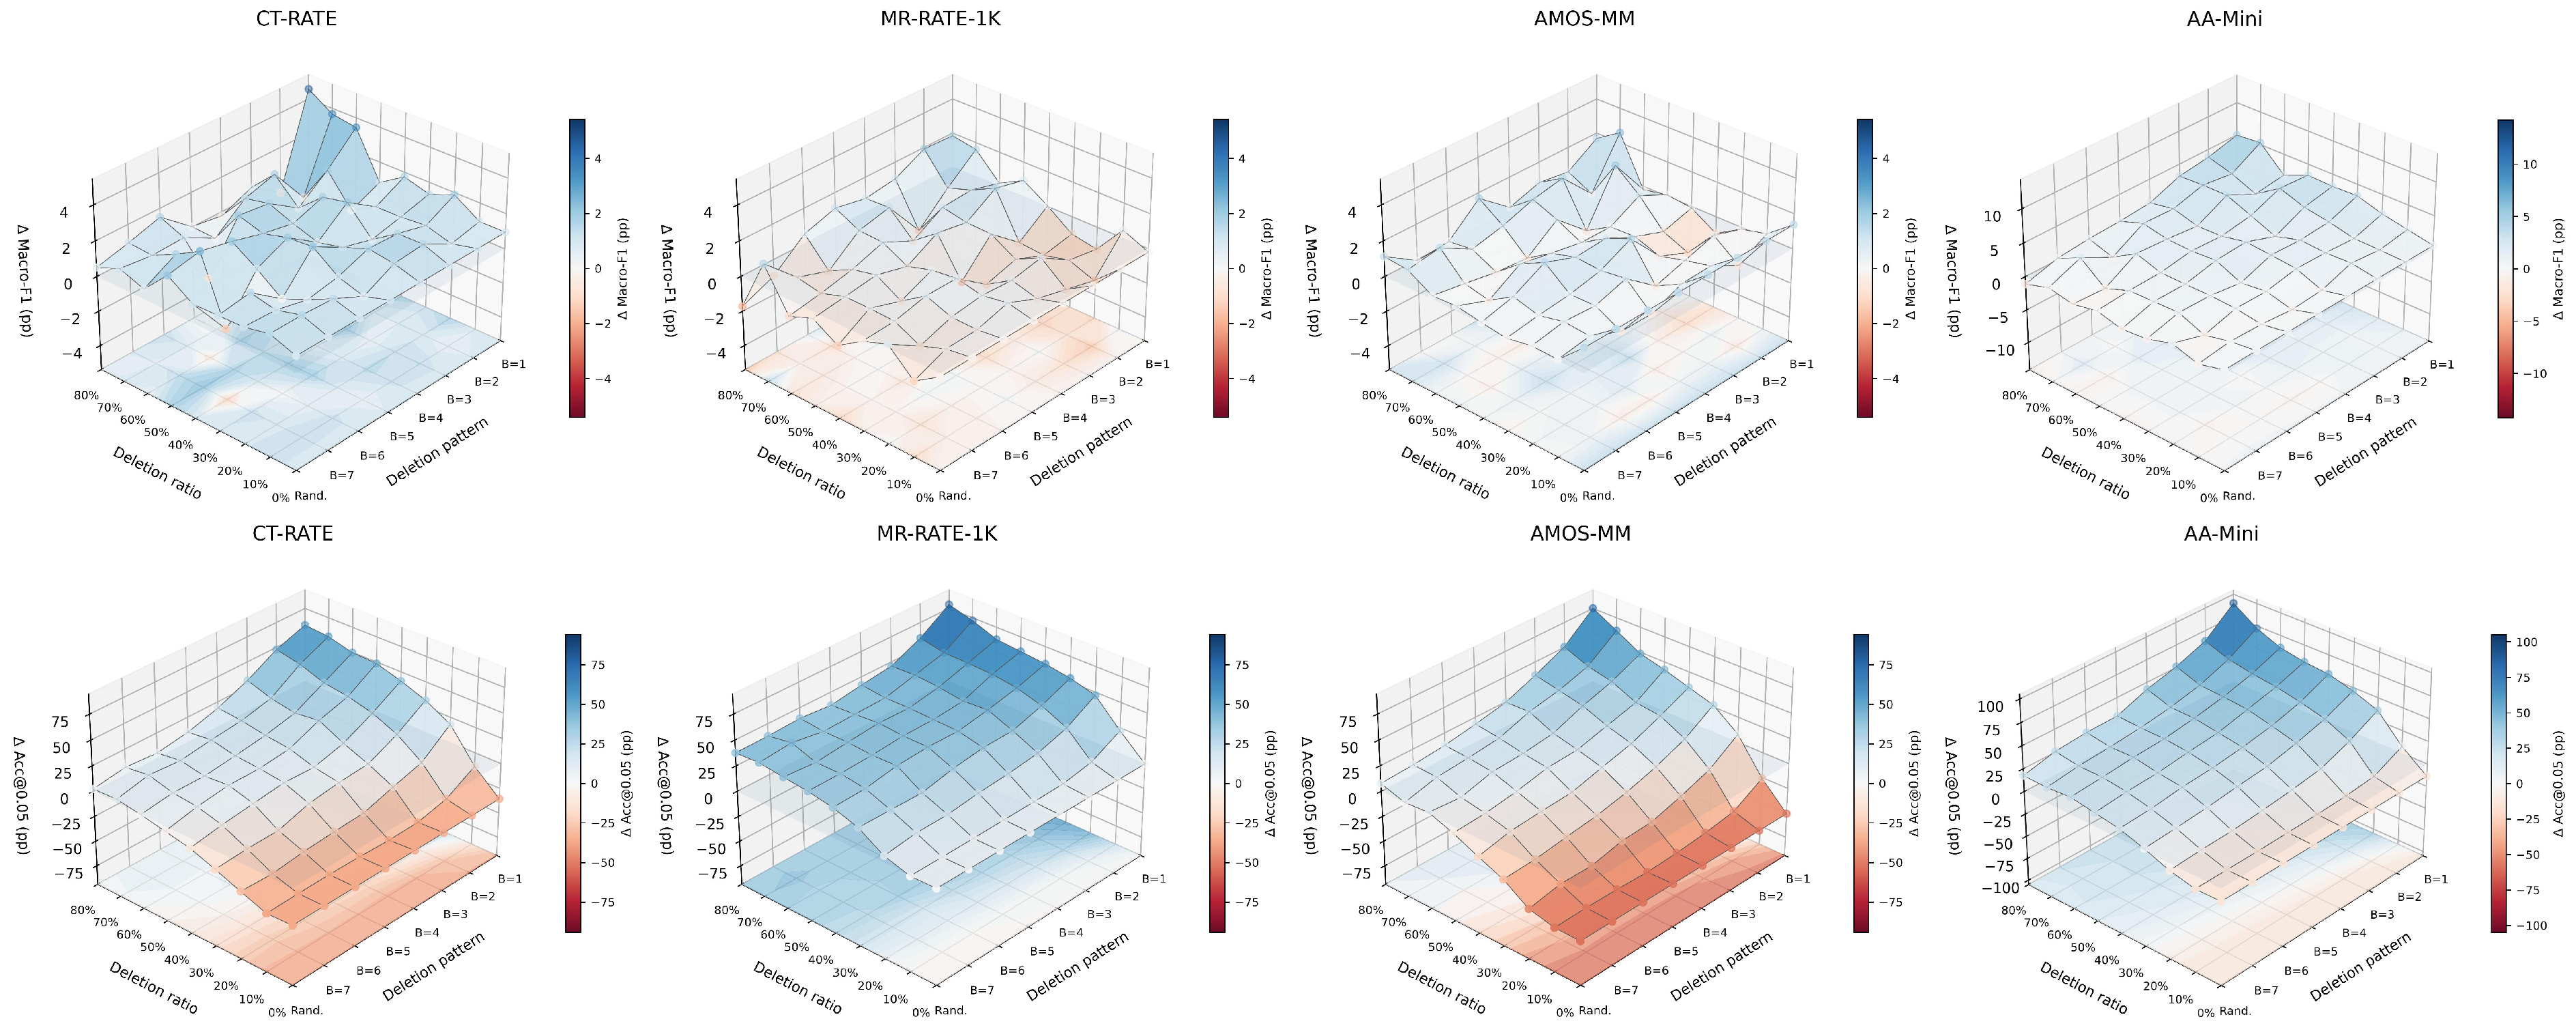
\includegraphics[width=\linewidth]{fig/fig3.pdf}
    \caption[Robustness under structured image missingness.]{%
        Structured image missingness on four public benchmarks.
        The top and bottom rows show ACPE--Original PE differences in F1 and Acc@0.05, respectively, in percentage points.
        Acc@0.05 measures agreement with acquisition indices using a normalized coordinate-error tolerance of 0.05.
        Blue and red indicate positive and negative differences.
        \cntranslation{%
            四个公开基准上的结构化图像缺失实验。上、下两行分别展示 F1 与 Acc@0.05 的差值，均为 ACPE 减去 Original PE，单位为百分点。Acc@0.05 衡量坐标与采集索引的一致性，允许的归一化坐标误差为 0.05。蓝色和红色分别表示正、负增益。
        }%
    }
    \label{fig:structured_missingness}
\end{figure}

% MR-RATE-1K 的趋势表述依据作者于 2026-09-29 确认的更新结果；当前图件后续替换。
To assess whether ACPE mitigates positional-reference mismatch under irregular sampling, we evaluate its robustness to structured image missingness on the four public datasets. We remove 0\%--80\% of images in 10-percentage-point increments, either uniformly at random or in $B\in\{1,\ldots,8\}$ contiguous blocks, and uniformly sample the remainder to provide identical inputs to ACPE and Original PE. As shown in Figure~\ref{fig:structured_missingness}, ACPE improves F1 in nearly all settings on CT-RATE and most settings on MR-RATE-1K, AMOS-MM, and AA-Mini, with a generally more pronounced advantage in relative position recovery under higher deletion ratios and more concentrated missingness. These results support ACPE's robustness to concentrated missingness, while its lower Acc@0.05 under mild, dispersed or no deletion can reflect adaptive shifts from acquisition references already well preserved by Original PE.

\cntranslation{%
为考察 ACPE 能否缓解不规则采样下的位置参照失配，我们在四个公开数据集上评估其对结构化图像缺失的鲁棒性。我们按 0\%--80\% 的比例（间隔 10 个百分点）随机删除图像或删除 $B\in\{1,\ldots,8\}$ 个连续块，再对剩余图像均匀采样，为 ACPE 和 Original PE 提供相同输入。如图~\ref{fig:structured_missingness} 所示，ACPE 在 CT-RATE 的几乎所有设置下均提高了 F1，并在 MR-RATE-1K、AMOS-MM 和 AA-Mini 的多数设置下取得 F1 增益，且删除比例越高、缺失越集中，ACPE 在恢复图像间相对位置关系方面的优势通常越明显。这些结果支持了 ACPE 对集中图像缺失的鲁棒性，而其在轻度零散或无删除时较低的 Acc@0.05 可能源于自适应调整偏离了 Original PE 原本已较好保持的采集位置参照。
}

\subsection{Analysis of ACPE}
\label{sec:acpe_analysis}

% 本节先记录对照设置与分析目的；所有结果留空，待作者确认数据后补写结论。
\paragraph{Comparison with positional modeling methods.}
To evaluate ACPE's improvements in classification performance for ordered images, we compare it with representative state-of-the-art positional modeling methods. We replace only the positional component in ALM-MIL with Original PE or one of ComRoPE-AP, VideoRoPE, PaTH, and DAPE V2-KERPLE. Table~\ref{tab:position_mechanism_comparison} reports the resulting five-fold F1 scores. ACPE ranks highest on all four public datasets, indicating that its contextual positional representation is more effective for this ordered multi-image setting than the alternative positional mechanisms.

\cntranslation{%
\textbf{位置建模方法比较。} 为评估 ACPE 在有序图像分类中的性能提升，我们将其与代表性的先进位置建模方法进行比较。我们仅在 ALM-MIL 中替换位置建模组件，分别采用 Original PE、ComRoPE-AP、VideoRoPE、PaTH 和 DAPE V2-KERPLE。表~\ref{tab:position_mechanism_comparison} 给出了五折 F1 结果。ACPE 在四个公开数据集上均取得最高结果，说明其上下文位置表征在当前有序多图像场景中比其他位置机制更有效。
}

\begin{table}[t]
\centering
\caption{Comparison of positional mechanisms (F1, \%). Results are reported as the five-fold mean $\pm$ standard deviation.}
\label{tab:position_mechanism_comparison}
\cntranslation{%
位置建模方法比较（F1，\%）。结果采用五折均值与标准差表示。
}
\setlength{\tabcolsep}{1.5pt}
\renewcommand{\arraystretch}{1.06}
\footnotesize
\begin{tabular*}{\linewidth}{@{\extracolsep{\fill}}l|cccc@{}}
\toprule
Method & {\fontsize{7.5}{8.5}\selectfont CT-RATE} & {\fontsize{7.5}{8.5}\selectfont MR-RATE-1K} & {\fontsize{7.5}{8.5}\selectfont AMOS-MM} & {\fontsize{7.5}{8.5}\selectfont AA-Mini} \\
\midrule
ComRoPE-AP~\cite{yu2025comrope} & 77.57\scalebox{0.6667}{$\pm$2.74} & 71.21\scalebox{0.6667}{$\pm$2.03} & 51.89\scalebox{0.6667}{$\pm$3.43} & 73.04\scalebox{0.6667}{${\pm}$1.75} \\
VideoRoPE~\cite{wei2025videorope} & 79.99\scalebox{0.6667}{$\pm$1.50} & 72.59\scalebox{0.6667}{$\pm$1.69} & 49.80\scalebox{0.6667}{$\pm$1.83} & 72.20\scalebox{0.6667}{${\pm}$1.45} \\
PaTH~\cite{yang2025path} & 77.77\scalebox{0.6667}{$\pm$2.89} & 71.69\scalebox{0.6667}{$\pm$2.11} & 52.47\scalebox{0.6667}{$\pm$3.62} & 72.69\scalebox{0.6667}{${\pm}$1.30} \\
DAPE V2-KERPLE~\cite{zheng2025dapev2} & 77.85\scalebox{0.6667}{$\pm$3.07} & 71.74\scalebox{0.6667}{$\pm$2.48} & 53.34\scalebox{0.6667}{$\pm$3.33} & 73.25\scalebox{0.6667}{${\pm}$0.80} \\
\midrule
\textbf{ACPE (Ours)} & \textbf{81.34\scalebox{0.6667}{$\pm$1.86}} & \textbf{74.45\scalebox{0.6667}{$\pm$1.93}} & \textbf{54.12\scalebox{0.6667}{$\pm$3.12}} & \textbf{73.85\scalebox{0.6667}{${\pm}$1.79}} \\
\bottomrule
\end{tabular*}
\end{table}

\paragraph{Contextual descriptor ablation.}
ACPE uses visual transitions to adjust neighboring intervals, so we ablate the descriptor components to identify their contributions. We vary the inclusion of the current-image feature, signed transitions, their magnitudes, and the cross-side interaction. Table~\ref{tab:transition_mlp_ablation} summarizes the corresponding descriptor ablations. The complete descriptor is strongest on CT-RATE, MR-RATE-1K, and AA-Mini, whereas reduced descriptors can be better on AMOS-MM, suggesting that the individual signals are complementary but their relative utility depends on the imaging distribution.

\cntranslation{%
\textbf{上下文描述子消融。} ACPE 利用视觉转变调整相邻间距，因此我们对描述子组成进行消融，以分析各部分的作用。我们改变当前图像特征、有符号转变、转变幅值和两侧交互项的组合。表~\ref{tab:transition_mlp_ablation} 汇总了相应的描述子消融结果。在 CT-RATE、MR-RATE-1K 和 AA-Mini 上，完整描述子取得最佳结果，而 AMOS-MM 上部分精简描述子更优，说明各信号具有互补作用，但其相对价值会随成像分布而变化。
}

\begin{table}[t]
\centering
\caption{Contextual descriptor ablation (F1, \%). Checkmarks indicate included groups; $\delta_{it}^{\pm}$ and $m_{it}^{\pm}$ each include both sides.}
\label{tab:transition_mlp_ablation}
\cntranslation{%
上下文描述子消融（F1，\%）。勾选表示包含相应信息组，$\delta_{it}^{\pm}$ 和 $m_{it}^{\pm}$ 均包含前后两侧信息。
}
\setlength{\tabcolsep}{1.5pt}
\renewcommand{\arraystretch}{1.06}
\footnotesize
\begin{tabular*}{\linewidth}{@{\extracolsep{\fill}}cccc|*{4}{c}@{}}
\toprule
$u_{it}$ & $\delta_{it}^{\pm}$ & $m_{it}^{\pm}$ & $q_{it}$ & {\fontsize{7.5}{8.5}\selectfont CT-RATE} & {\fontsize{7.5}{8.5}\selectfont MR-RATE-1K} & {\fontsize{7.5}{8.5}\selectfont AMOS-MM} & {\fontsize{7.5}{8.5}\selectfont AA-Mini} \\
\midrule
$\checkmark$ & $\times$ & $\times$ & $\times$ & 77.58\scalebox{0.6667}{$\pm$0.53} & 73.20\scalebox{0.6667}{$\pm$2.65} & \textbf{55.44\scalebox{0.6667}{$\pm$3.46}} & 72.68\scalebox{0.6667}{${\pm}$1.18} \\
$\checkmark$ & $\checkmark$ & $\times$ & $\times$ & 79.57\scalebox{0.6667}{$\pm$1.76} & 73.44\scalebox{0.6667}{$\pm$1.33} & 54.31\scalebox{0.6667}{$\pm$3.69} & 72.05\scalebox{0.6667}{${\pm}$1.79} \\
$\checkmark$ & $\times$ & $\checkmark$ & $\times$ & 79.47\scalebox{0.6667}{$\pm$2.10} & 71.77\scalebox{0.6667}{$\pm$2.77} & 52.93\scalebox{0.6667}{$\pm$2.15} & 71.71\scalebox{0.6667}{${\pm}$0.59} \\
$\checkmark$ & $\checkmark$ & $\times$ & $\checkmark$ & 77.62\scalebox{0.6667}{$\pm$2.18} & 71.45\scalebox{0.6667}{$\pm$3.69} & 53.42\scalebox{0.6667}{$\pm$4.01} & 73.42\scalebox{0.6667}{${\pm}$2.32} \\
$\checkmark$ & $\times$ & $\checkmark$ & $\checkmark$ & 80.51\scalebox{0.6667}{$\pm$3.16} & 71.84\scalebox{0.6667}{$\pm$2.44} & 52.62\scalebox{0.6667}{$\pm$4.92} & 73.17\scalebox{0.6667}{${\pm}$1.73} \\
$\times$ & $\checkmark$ & $\checkmark$ & $\checkmark$ & 78.94\scalebox{0.6667}{$\pm$2.38} & 72.90\scalebox{0.6667}{$\pm$1.48} & 55.20\scalebox{0.6667}{$\pm$1.96} & 72.91\scalebox{0.6667}{${\pm}$1.38} \\
\midrule
$\checkmark$ & $\checkmark$ & $\checkmark$ & $\checkmark$ & \textbf{81.34\scalebox{0.6667}{$\pm$1.86}} & \textbf{74.45\scalebox{0.6667}{$\pm$1.93}} & 54.12\scalebox{0.6667}{$\pm$3.12} & \textbf{73.85\scalebox{0.6667}{${\pm}$1.79}} \\
\bottomrule
\end{tabular*}
\end{table}

\paragraph{Position-injection route ablation.}
We observe that, with all images retained, ACPE exhibits pronounced over-correction relative to Original PE yet achieves a higher F1. This suggests that the absolute and relative injection routes may provide complementary benefits, so we evaluate each route separately and their combination. Table~\ref{tab:position_route_ablation} reports the resulting F1 scores. Combining both routes gives the strongest result on every dataset, showing that absolute coordinate features and relative attention biases contribute distinct information and can improve recognition even when coordinate agreement with the raw acquisition reference is not maximal.

\cntranslation{%
\textbf{位置注入路径消融。} 我们观察到，在保留全部图像时，ACPE 相比 Original PE 存在明显的过度修正现象，却取得了更高的 F1。这表明绝对路径和相对路径可能提供互补的识别收益，因此我们分别评估两条路径及其组合。表~\ref{tab:position_route_ablation} 给出了相应的 F1 结果。两条路径结合时在所有数据集上均取得最强结果，表明绝对坐标特征与相对注意力偏置提供了不同信息，即使坐标与原始采集参照的一致性并非最高，也能够提升识别性能。
}

\begin{table}[t]
\centering
\caption{Position-injection route ablation (F1, \%). Abs. and Rel. denote the absolute and relative routes.}
\label{tab:position_route_ablation}
\cntranslation{%
位置注入路径消融（F1，\%）。Abs. 和 Rel. 分别表示绝对路径与相对路径。
}
\setlength{\tabcolsep}{1.5pt}
\renewcommand{\arraystretch}{1.06}
\footnotesize
\begin{tabular*}{\linewidth}{@{\extracolsep{\fill}}cc|*{4}{c}@{}}
\toprule
Abs. & Rel. & {\fontsize{7.5}{8.5}\selectfont CT-RATE} & {\fontsize{7.5}{8.5}\selectfont MR-RATE-1K} & {\fontsize{7.5}{8.5}\selectfont AMOS-MM} & {\fontsize{7.5}{8.5}\selectfont AA-Mini} \\
\midrule
$\checkmark$ & $\times$ & 79.43\scalebox{0.6667}{$\pm$1.99} & 71.39\scalebox{0.6667}{$\pm$1.64} & 52.59\scalebox{0.6667}{$\pm$4.49} & 72.80\scalebox{0.6667}{${\pm}$1.75} \\
$\times$ & $\checkmark$ & 77.53\scalebox{0.6667}{$\pm$2.40} & 71.44\scalebox{0.6667}{$\pm$2.09} & 52.40\scalebox{0.6667}{$\pm$2.13} & 72.80\scalebox{0.6667}{${\pm}$1.75} \\
\midrule
$\checkmark$ & $\checkmark$ & \textbf{81.34\scalebox{0.6667}{$\pm$1.86}} & \textbf{74.45\scalebox{0.6667}{$\pm$1.93}} & \textbf{54.12\scalebox{0.6667}{$\pm$3.12}} & \textbf{73.85\scalebox{0.6667}{${\pm}$1.79}} \\
\bottomrule
\end{tabular*}
\end{table}

\subsection{Analysis of LCCF}
\label{sec:lccf_analysis}

\begin{figure}[t]
    \centering
    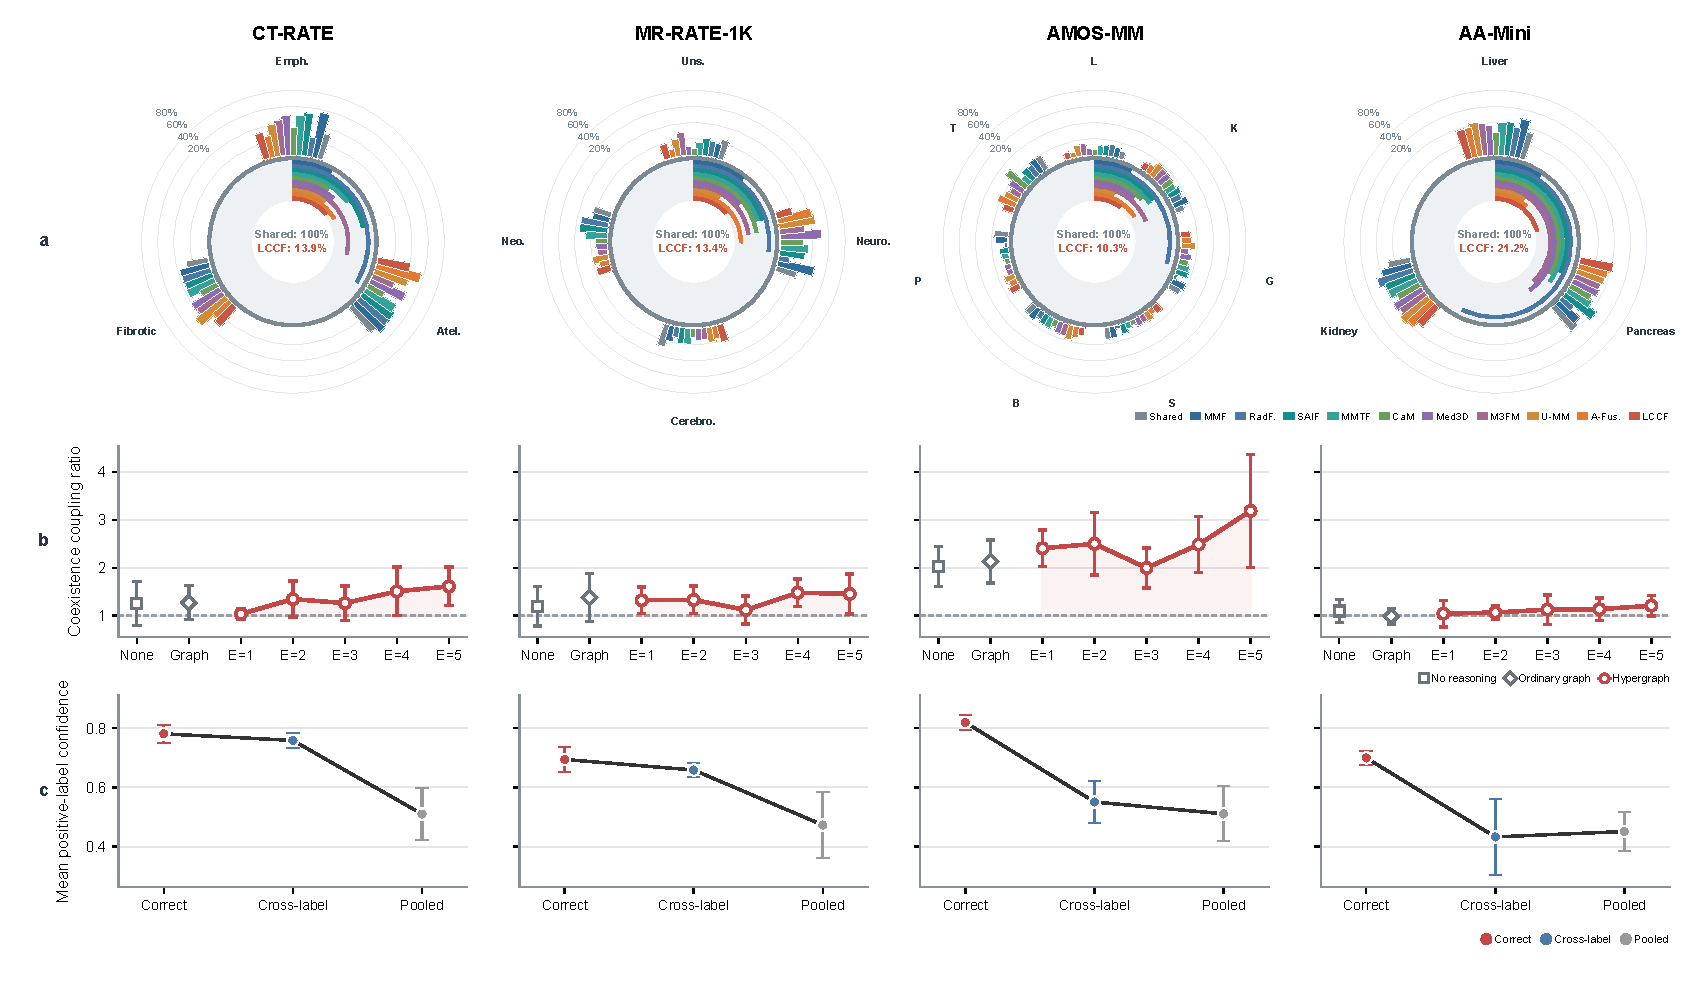
\includegraphics[width=\linewidth]{fig/fig4.pdf}
    \caption[Analysis of label-centric multimodal evidence.]{%
        Analysis of label-centric multimodal evidence on four public datasets.
        (a) Label-wise image occupancy and overlap with the shared-control
        attention; (b) coexistence coupling under no reasoning, an ordinary
        graph, and hypergraph reasoning with different numbers of hyperedges;
        (c) mean positive-label confidence under correct, cross-label, and
        pooled textual evidence.\cntranslation{%
        四个公开数据集上的标签中心多模态证据分析。(a) 标签级图像占有率及其与共享控制注意力的重叠程度；(b) 无推理、普通图结构和不同超边数量的超图推理下的共存耦合；(c) 正确、跨标签及共享文本证据下的平均正标签置信度。}%
    }
    \label{fig:lccf_analysis}
\end{figure}

\paragraph{Label-specific visual evidence.}
Different labels within the same examination may rely on different images, yet
many multimodal baselines assign multiple labels to highly overlapping image
subsets.  To examine whether LCCF addresses this issue, we measure the pairwise
overlap among label-wise selected image sets and compare LCCF with alternative
visual aggregation strategies within the same framework.  The results are
presented in Fig.~\ref{fig:lccf_analysis}(a) and
Table~\ref{tab:lccf_visual_ablation}.  Across all four public datasets, LCCF is
among the few methods with the lowest overlap rates.  On AA-Mini, many
multimodal baselines struggle to capture the weak label co-occurrence structure
and consequently assign multiple labels to common images, leading to higher
overlap, whereas LCCF still maintains low overlap; the complete label-wise
aggregator also achieves the highest F1 among the LCCF variants.  Together,
these results show that LCCF allows different labels to select distinct image
evidence while preserving label-specific visual organization across datasets.

\cntranslation{%
\textbf{标签特异性视觉证据。}
同一次检查中的不同标签可能依赖不同图像，但许多多模态基线会让多个标签使用高度重叠的图像集合。为了查看 LCCF 是否解决了这一问题，我们统计标签级图像选择之间的成对重叠率，并在相同框架下比较 LCCF 与不同视觉聚合方式的表现。结果如图~\ref{fig:lccf_analysis}(a) 和表~\ref{tab:lccf_visual_ablation} 所示。在四个公开数据集中，LCCF 均属于重叠率最低的几个方法之一。尤其是在 AA-Mini 上，许多多模态基线难以捕捉较弱的标签共现关系，因而倾向于让多个标签依赖共同图像并产生更高的重叠率，而 LCCF 仍保持较低的重叠率；同时，完整的标签级聚合在 LCCF 的各个变体中取得了最高 F1。综合来看，LCCF 能够使不同标签选择具有区分性的图像证据，并在不同数据集上保持标签特异性的视觉组织能力。
}

\begin{table}[t]
\centering
\caption{Visual aggregation ablation in LCCF (F1, \%). Mean, Max, and Shared-Attn denote mean pooling, max pooling, and shared attention, respectively.}
\label{tab:lccf_visual_ablation}
\cntranslation{%
LCCF 视觉聚合消融（F1，\%）。Mean、Max 和 Shared-Attn 分别表示均值池化、最大池化和共享注意力。
}
\setlength{\tabcolsep}{1.8pt}
\renewcommand{\arraystretch}{1.06}
\footnotesize
\begin{tabular*}{\linewidth}{@{\extracolsep{\fill}}l|*{4}{c}@{}}
\toprule
Variant & {\fontsize{7.5}{8.5}\selectfont CT-RATE} & {\fontsize{7.5}{8.5}\selectfont MR-RATE-1K} & {\fontsize{7.5}{8.5}\selectfont AMOS-MM} & {\fontsize{7.5}{8.5}\selectfont AA-Mini} \\
\midrule
Mean & 78.76\scalebox{0.6667}{$\pm$4.11} & 72.43\scalebox{0.6667}{$\pm$2.27} & 53.39\scalebox{0.6667}{$\pm$5.68} & 72.81\scalebox{0.6667}{$\pm$0.89} \\
Max & 67.22\scalebox{0.6667}{$\pm$13.26} & 64.03\scalebox{0.6667}{$\pm$1.44} & 42.27\scalebox{0.6667}{$\pm$1.76} & 63.27\scalebox{0.6667}{$\pm$1.43} \\
Shared-Attn & 79.66\scalebox{0.6667}{$\pm$1.34} & 71.15\scalebox{0.6667}{$\pm$2.72} & 53.23\scalebox{0.6667}{$\pm$3.98} & 72.12\scalebox{0.6667}{$\pm$0.84} \\
\midrule
\textbf{Label-Attn (Ours)} & \textbf{81.34\scalebox{0.6667}{$\pm$1.86}} & \textbf{74.45\scalebox{0.6667}{$\pm$1.93}} & \textbf{54.12\scalebox{0.6667}{$\pm$3.12}} & \textbf{73.85\scalebox{0.6667}{$\pm$1.79}} \\
\bottomrule
\end{tabular*}
\end{table}

\paragraph{Coexistence-aware label reasoning.}
Coexisting findings are not independent, so treating every label separately can
miss information shared by correlated abnormalities.  We compare no reasoning,
an ordinary label graph, and hypergraph variants with different numbers of latent
hyperedges; Figure~\ref{fig:lccf_analysis}(b) measures the resulting coexistence
coupling, while Table~\ref{tab:lccf_reasoning_ablation} reports the corresponding
F1 scores.  Hypergraph reasoning generally produces stronger coupling than the
non-reasoning and ordinary-graph alternatives.  Although some hypergraph
settings achieve higher F1 on individual datasets, HG-2 provides the most
consistent overall performance, supporting higher-order information exchange
while retaining label-specific representations.

\cntranslation{%
\textbf{共存感知标签推理。}
共存异常并非彼此独立，将每个标签完全分开处理可能忽略相关异常之间的共享信息。我们比较无推理、普通标签图以及不同潜在超边数量的超图变体；图~\ref{fig:lccf_analysis}(b) 衡量由此产生的共存耦合，表~\ref{tab:lccf_reasoning_ablation} 给出相应的 F1 结果。与无推理和普通图结构相比，超图推理通常产生更强的标签耦合。尽管部分超图设置在个别数据集上取得了更高的 F1，HG-2 在不同数据集上表现出更稳定的整体性能，说明在保留标签特异性表征的同时交换高阶信息是有益的。
}

\begin{table}[t]
\centering
\caption{Label reasoning ablation in LCCF (F1, \%). None denotes no label reasoning, Graph denotes an ordinary label graph, and HG-$E$ denotes a hypergraph with $E$ latent hyperedges.}
\label{tab:lccf_reasoning_ablation}
\cntranslation{%
LCCF 标签推理消融（F1，\%）。None 表示不进行标签推理，Graph 表示普通标签图，HG-$E$ 表示使用 $E$ 条潜在超边的超图。
}
\setlength{\tabcolsep}{1.8pt}
\renewcommand{\arraystretch}{1.06}
\footnotesize
\begin{tabular*}{\linewidth}{@{\extracolsep{\fill}}l|*{4}{c}@{}}
\toprule
Variant & {\fontsize{7.5}{8.5}\selectfont CT-RATE} & {\fontsize{7.5}{8.5}\selectfont MR-RATE-1K} & {\fontsize{7.5}{8.5}\selectfont AMOS-MM} & {\fontsize{7.5}{8.5}\selectfont AA-Mini} \\
\midrule
None & 80.22\scalebox{0.6667}{$\pm$2.89} & 72.23\scalebox{0.6667}{$\pm$2.70} & 52.36\scalebox{0.6667}{$\pm$2.91} & 72.61\scalebox{0.6667}{$\pm$2.32} \\
Graph & 78.54\scalebox{0.6667}{$\pm$4.18} & 71.51\scalebox{0.6667}{$\pm$2.86} & 52.10\scalebox{0.6667}{$\pm$3.65} & 72.48\scalebox{0.6667}{$\pm$1.23} \\
HG-1 & 81.20\scalebox{0.6667}{$\pm$1.58} & 72.15\scalebox{0.6667}{$\pm$1.72} & 51.87\scalebox{0.6667}{$\pm$4.01} & 71.68\scalebox{0.6667}{$\pm$1.70} \\
\textbf{HG-2 (Ours)} & \textbf{81.34\scalebox{0.6667}{$\pm$1.86}} & \textbf{74.45\scalebox{0.6667}{$\pm$1.93}} & 54.12\scalebox{0.6667}{$\pm$3.12} & \textbf{73.85\scalebox{0.6667}{$\pm$1.79}} \\
HG-3 & 79.11\scalebox{0.6667}{$\pm$1.87} & 72.97\scalebox{0.6667}{$\pm$2.17} & 51.70\scalebox{0.6667}{$\pm$2.46} & 72.36\scalebox{0.6667}{$\pm$1.25} \\
HG-4 & 79.85\scalebox{0.6667}{$\pm$3.55} & 71.67\scalebox{0.6667}{$\pm$3.04} & \textbf{54.39\scalebox{0.6667}{$\pm$1.17}} & 71.74\scalebox{0.6667}{$\pm$0.95} \\
HG-5 & 80.31\scalebox{0.6667}{$\pm$2.56} & 71.81\scalebox{0.6667}{$\pm$2.32} & 52.98\scalebox{0.6667}{$\pm$3.03} & 72.29\scalebox{0.6667}{$\pm$2.19} \\
\bottomrule
\end{tabular*}
\end{table}

\paragraph{Label-conditioned textual evidence integration.}
A paired report can contain evidence for several findings, so a shared report
vector or indiscriminate fusion may mix label-matched and label-mismatched
information.  To examine whether LCCF retrieves and injects label-appropriate
textual evidence, we compare correct, cross-label, and pooled textual evidence
in Fig.~\ref{fig:lccf_analysis}(c), and evaluate label-conditioned retrieval and
adaptive fusion in Tables~\ref{tab:lccf_text_ablation} and
\ref{tab:lccf_fusion_ablation}.  On CT-RATE, MR-RATE-1K, and AMOS-MM, correct
evidence produces the highest positive-label confidence, while cross-label
evidence remains more informative than pooled evidence, suggesting that label
co-occurrence can provide indirect textual cues across findings.  AA-Mini shows
the opposite ordering, with cross-label confidence lower than pooled confidence.
In AA-Mini, weak label co-occurrence provides little cross-label textual cue,
causing cross-label evidence to perform worse than the pooled representation.
Although
individual retrieval or fusion alternatives can achieve higher F1 on particular
datasets, the complete label-conditioned design remains competitive across
datasets.  These results show that LCCF benefits from matching textual evidence
to each label and adapting its contribution to the available label relationships.

\cntranslation{%
\textbf{标签条件文本证据整合。}
一份配对报告可能同时包含多个异常的相关信息，因此共享报告向量或无差别融合容易混合与标签匹配和不匹配的文本。为考察 LCCF 是否能够检索并注入与标签匹配的文本证据，我们在图~\ref{fig:lccf_analysis}(c) 中比较正确、跨标签和共享文本证据，并在表~\ref{tab:lccf_text_ablation} 和表~\ref{tab:lccf_fusion_ablation} 中评估标签条件检索与自适应融合。在 CT-RATE、MR-RATE-1K 和 AMOS-MM 上，正确文本证据带来的正标签置信度最高，而跨标签证据仍然比共享证据更有信息量，说明标签共现关系可能使报告中的文本为其他异常提供间接提示。AA-Mini 则呈现相反的排序，跨标签置信度低于共享证据。在 AA-Mini 中，较弱的标签共现关系难以提供充分的跨标签文本提示，因此跨标签证据的表现低于保留报告整体信息的共享表征。尽管个别文本检索或融合替代方案在某些数据集上可以取得更高的 F1，完整的标签条件设计在不同数据集上仍保持了有竞争力的表现。上述结果表明，LCCF 能够将文本证据匹配到对应标签，并根据可利用的标签关系自适应地调节其贡献。
}

\begin{table}[t]
\centering
\caption{Text retrieval ablation in LCCF (F1, \%). Mean denotes mean text retrieval, Shared-Q a shared query, and Label-Q a label-wise query without label identity.}
\label{tab:lccf_text_ablation}
\cntranslation{%
LCCF 文本检索消融（F1，\%）。Mean 表示均值文本检索，Shared-Q 表示共享查询，Label-Q 表示不含标签身份的标签级查询。
}
\setlength{\tabcolsep}{1.8pt}
\renewcommand{\arraystretch}{1.06}
\footnotesize
\begin{tabular*}{\linewidth}{@{\extracolsep{\fill}}l|*{4}{c}@{}}
\toprule
Variant & {\fontsize{7.5}{8.5}\selectfont CT-RATE} & {\fontsize{7.5}{8.5}\selectfont MR-RATE-1K} & {\fontsize{7.5}{8.5}\selectfont AMOS-MM} & {\fontsize{7.5}{8.5}\selectfont AA-Mini} \\
\midrule
Mean & 61.13\scalebox{0.6667}{$\pm$2.94} & 71.11\scalebox{0.6667}{$\pm$1.61} & 49.70\scalebox{0.6667}{$\pm$0.66} & 71.04\scalebox{0.6667}{$\pm$2.15} \\
Shared-Q & 79.77\scalebox{0.6667}{$\pm$2.82} & 72.01\scalebox{0.6667}{$\pm$1.63} & \textbf{55.93\scalebox{0.6667}{$\pm$3.61}} & 72.43\scalebox{0.6667}{$\pm$0.50} \\
Label-Q & 78.47\scalebox{0.6667}{$\pm$2.45} & 71.04\scalebox{0.6667}{$\pm$1.80} & 51.85\scalebox{0.6667}{$\pm$3.79} & 72.49\scalebox{0.6667}{$\pm$1.15} \\
\midrule
\textbf{Label-query (Ours)} & \textbf{81.34\scalebox{0.6667}{$\pm$1.86}} & \textbf{74.45\scalebox{0.6667}{$\pm$1.93}} & 54.12\scalebox{0.6667}{$\pm$3.12} & \textbf{73.85\scalebox{0.6667}{$\pm$1.79}} \\
\bottomrule
\end{tabular*}
\end{table}

\begin{table}[t]
\centering
\caption{Fusion ablation in LCCF (F1, \%). Add denotes direct addition, Fixed a fixed gate value of 0.5, L-Gate a label-wise constant gate, and E-Gate an examination-wise shared gate.}
\label{tab:lccf_fusion_ablation}
\cntranslation{%
LCCF 融合消融（F1，\%）。Add 表示直接相加，Fixed 表示门控值固定为 0.5，L-Gate 表示标签级恒定门控，E-Gate 表示检查级共享门控。
}
\setlength{\tabcolsep}{1.8pt}
\renewcommand{\arraystretch}{1.06}
\footnotesize
\begin{tabular*}{\linewidth}{@{\extracolsep{\fill}}l|*{4}{c}@{}}
\toprule
Variant & {\fontsize{7.5}{8.5}\selectfont CT-RATE} & {\fontsize{7.5}{8.5}\selectfont MR-RATE-1K} & {\fontsize{7.5}{8.5}\selectfont AMOS-MM} & {\fontsize{7.5}{8.5}\selectfont AA-Mini} \\
\midrule
Add & 78.60\scalebox{0.6667}{$\pm$5.52} & 72.51\scalebox{0.6667}{$\pm$2.06} & 53.24\scalebox{0.6667}{$\pm$1.97} & 72.60\scalebox{0.6667}{$\pm$2.18} \\
Fixed & \textbf{82.36\scalebox{0.6667}{$\pm$2.49}} & 70.26\scalebox{0.6667}{$\pm$2.76} & 52.21\scalebox{0.6667}{$\pm$5.21} & 72.54\scalebox{0.6667}{$\pm$2.04} \\
L-Gate & 81.11\scalebox{0.6667}{$\pm$3.90} & 72.53\scalebox{0.6667}{$\pm$1.74} & 50.40\scalebox{0.6667}{$\pm$4.21} & 73.61\scalebox{0.6667}{$\pm$0.85} \\
E-Gate & 79.76\scalebox{0.6667}{$\pm$1.88} & 73.97\scalebox{0.6667}{$\pm$1.00} & \textbf{55.49\scalebox{0.6667}{$\pm$1.09}} & 72.04\scalebox{0.6667}{$\pm$1.75} \\
\midrule
\textbf{Adaptive gate (Ours)} & 81.34\scalebox{0.6667}{$\pm$1.86} & \textbf{74.45\scalebox{0.6667}{$\pm$1.93}} & 54.12\scalebox{0.6667}{$\pm$3.12} & \textbf{73.85\scalebox{0.6667}{$\pm$1.79}} \\
\bottomrule
\end{tabular*}
\end{table}
